% Options for packages loaded elsewhere
\PassOptionsToPackage{unicode}{hyperref}
\PassOptionsToPackage{hyphens}{url}
%
\documentclass[
]{book}
\usepackage{lmodern}
\usepackage{amsmath}
\usepackage{ifxetex,ifluatex}
\ifnum 0\ifxetex 1\fi\ifluatex 1\fi=0 % if pdftex
  \usepackage[T1]{fontenc}
  \usepackage[utf8]{inputenc}
  \usepackage{textcomp} % provide euro and other symbols
  \usepackage{amssymb}
\else % if luatex or xetex
  \usepackage{unicode-math}
  \defaultfontfeatures{Scale=MatchLowercase}
  \defaultfontfeatures[\rmfamily]{Ligatures=TeX,Scale=1}
\fi
% Use upquote if available, for straight quotes in verbatim environments
\IfFileExists{upquote.sty}{\usepackage{upquote}}{}
\IfFileExists{microtype.sty}{% use microtype if available
  \usepackage[]{microtype}
  \UseMicrotypeSet[protrusion]{basicmath} % disable protrusion for tt fonts
}{}
\makeatletter
\@ifundefined{KOMAClassName}{% if non-KOMA class
  \IfFileExists{parskip.sty}{%
    \usepackage{parskip}
  }{% else
    \setlength{\parindent}{0pt}
    \setlength{\parskip}{6pt plus 2pt minus 1pt}}
}{% if KOMA class
  \KOMAoptions{parskip=half}}
\makeatother
\usepackage{xcolor}
\IfFileExists{xurl.sty}{\usepackage{xurl}}{} % add URL line breaks if available
\IfFileExists{bookmark.sty}{\usepackage{bookmark}}{\usepackage{hyperref}}
\hypersetup{
  pdftitle={TD's: Résistances de Matériaux - EEIGM - ENSGSI},
  pdfauthor={Olivier FARGE, Fangkai XUE et Fabio CRUZ},
  hidelinks,
  pdfcreator={LaTeX via pandoc}}
\urlstyle{same} % disable monospaced font for URLs
\usepackage{longtable,booktabs}
\usepackage{calc} % for calculating minipage widths
% Correct order of tables after \paragraph or \subparagraph
\usepackage{etoolbox}
\makeatletter
\patchcmd\longtable{\par}{\if@noskipsec\mbox{}\fi\par}{}{}
\makeatother
% Allow footnotes in longtable head/foot
\IfFileExists{footnotehyper.sty}{\usepackage{footnotehyper}}{\usepackage{footnote}}
\makesavenoteenv{longtable}
\usepackage{graphicx}
\makeatletter
\def\maxwidth{\ifdim\Gin@nat@width>\linewidth\linewidth\else\Gin@nat@width\fi}
\def\maxheight{\ifdim\Gin@nat@height>\textheight\textheight\else\Gin@nat@height\fi}
\makeatother
% Scale images if necessary, so that they will not overflow the page
% margins by default, and it is still possible to overwrite the defaults
% using explicit options in \includegraphics[width, height, ...]{}
\setkeys{Gin}{width=\maxwidth,height=\maxheight,keepaspectratio}
% Set default figure placement to htbp
\makeatletter
\def\fps@figure{htbp}
\makeatother
\setlength{\emergencystretch}{3em} % prevent overfull lines
\providecommand{\tightlist}{%
  \setlength{\itemsep}{0pt}\setlength{\parskip}{0pt}}
\setcounter{secnumdepth}{5}
\usepackage{booktabs}
\usepackage{amsmath}
\ifluatex
  \usepackage{selnolig}  % disable illegal ligatures
\fi
\usepackage[]{natbib}
\bibliographystyle{apalike}

\title{TD's: Résistances de Matériaux - EEIGM - ENSGSI}
\author{Olivier FARGE, Fangkai XUE et Fabio CRUZ}
\date{2021-01-17}

\begin{document}
\maketitle

{
\setcounter{tocdepth}{1}
\tableofcontents
}
\hypertarget{ruxe9sistances-des-matuxe9riaux}{%
\chapter*{Résistances des Matériaux}\label{ruxe9sistances-des-matuxe9riaux}}
\addcontentsline{toc}{chapter}{Résistances des Matériaux}

\hypertarget{planning}{%
\section*{Planning}\label{planning}}
\addcontentsline{toc}{section}{Planning}

\begin{center}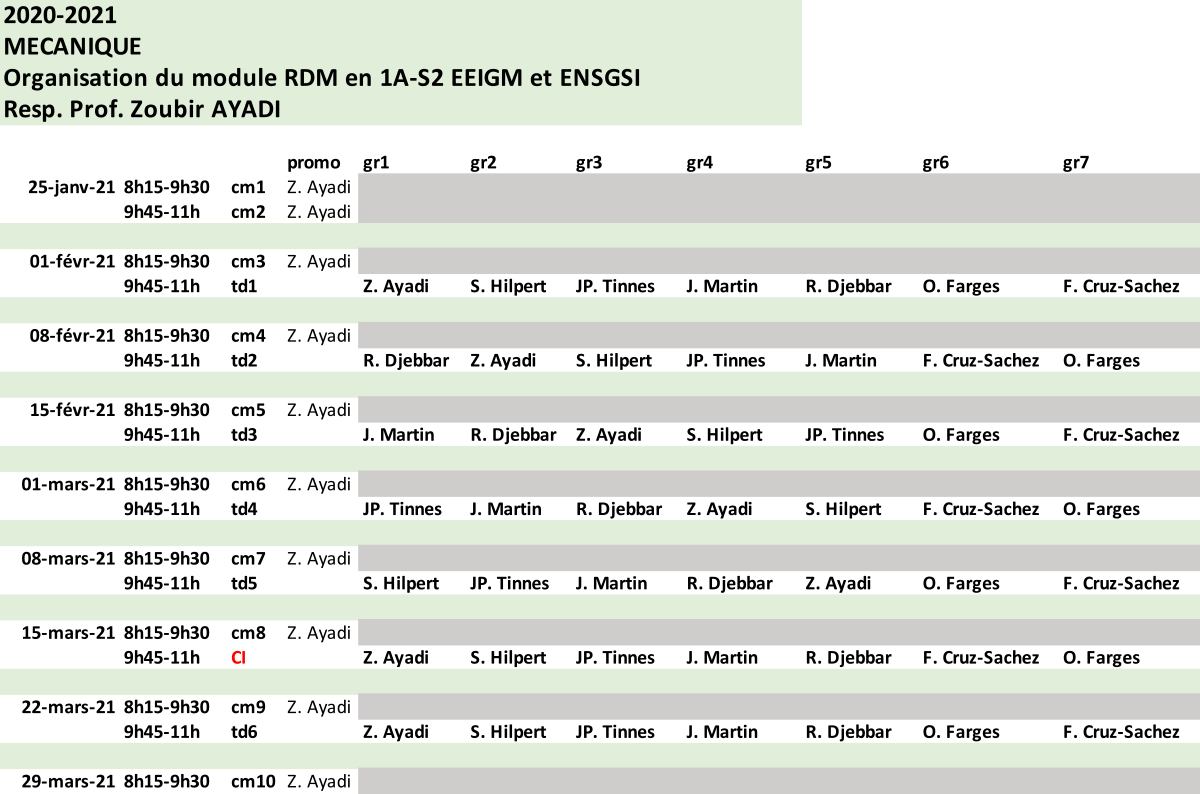
\includegraphics[width=600pt]{Figures/Organization-01} \end{center}

\begin{center}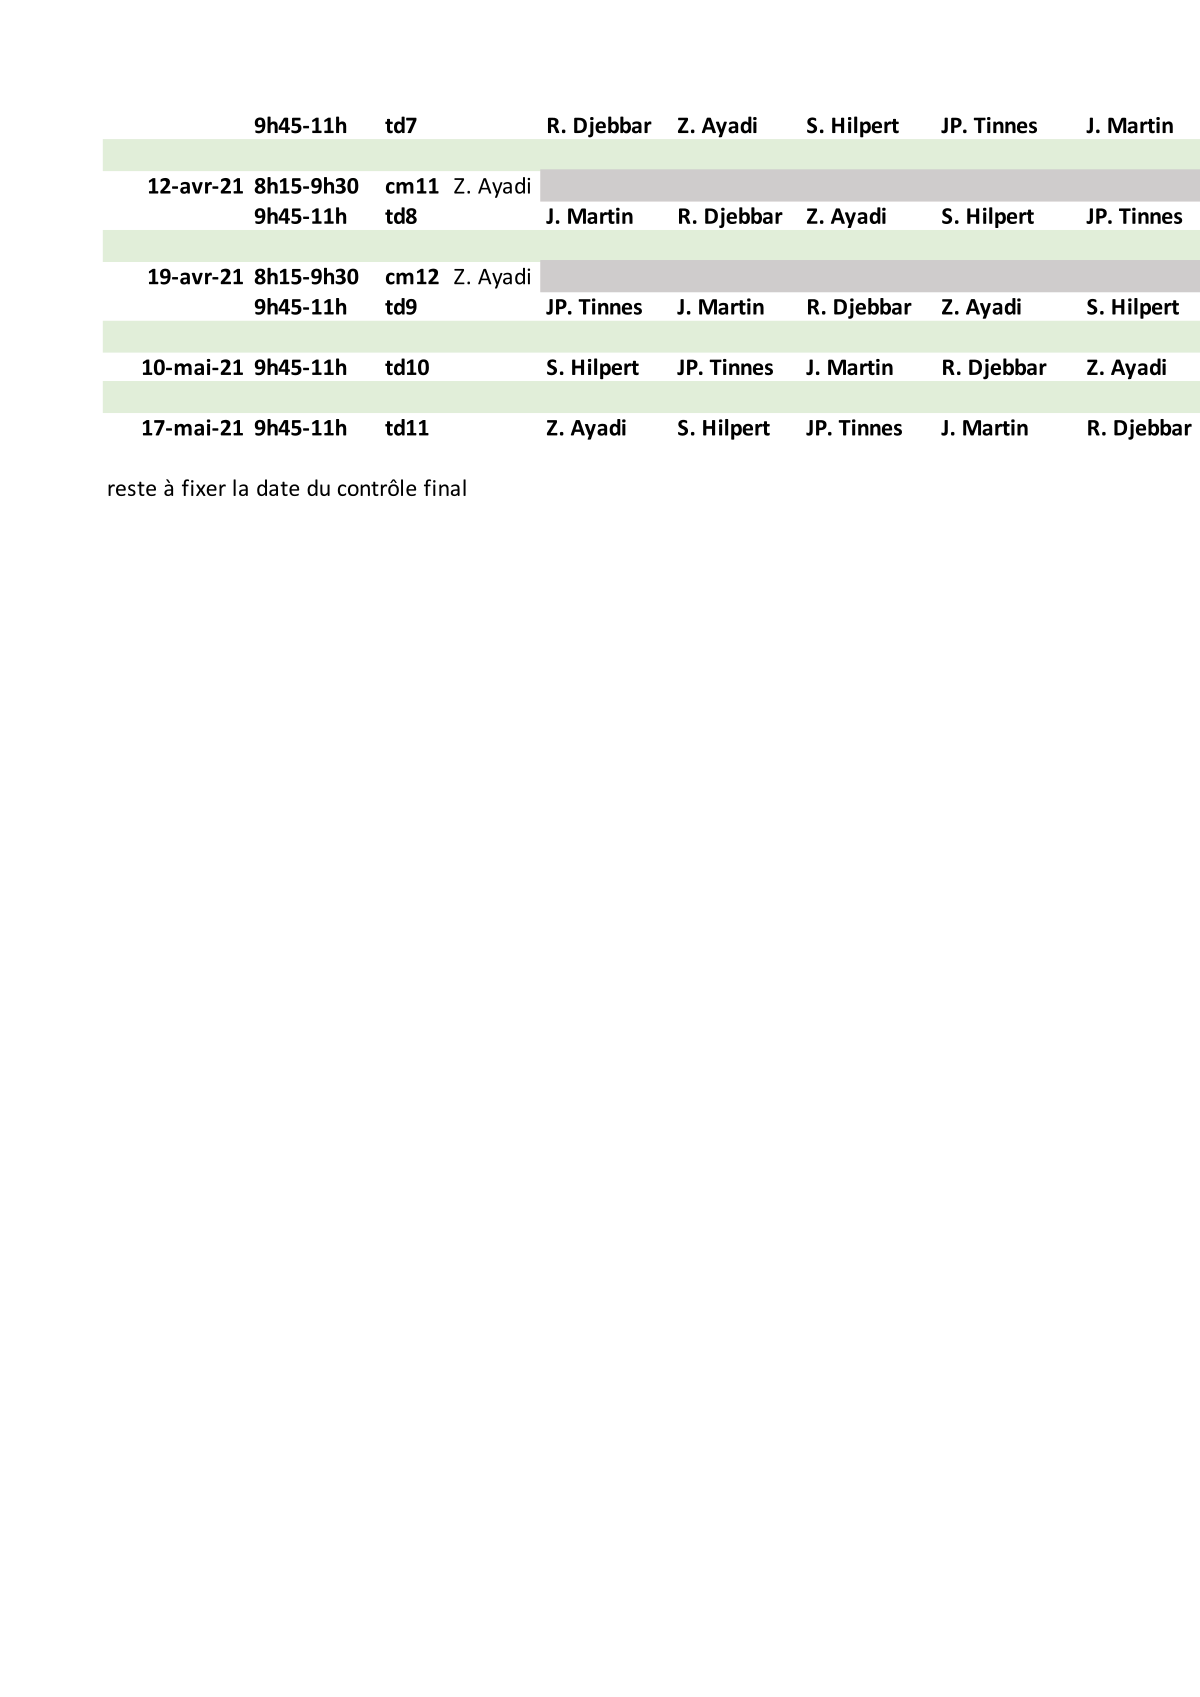
\includegraphics[width=600pt]{Figures/Organization-02} \end{center}

\hypertarget{introduction}{%
\chapter*{Introduction}\label{introduction}}
\addcontentsline{toc}{chapter}{Introduction}

\hypertarget{plan-du-cours}{%
\section*{Plan du cours}\label{plan-du-cours}}
\addcontentsline{toc}{section}{Plan du cours}

\begin{enumerate}
\def\labelenumi{\arabic{enumi}.}
\tightlist
\item
  Introduction
\end{enumerate}

\begin{itemize}
\tightlist
\item
  Modalités de déroulemen et validation du module RDM
\item
  La Mécanique, la Résistances des Matériaux
\item
  Dimensionnement des structures
\end{itemize}

\begin{enumerate}
\def\labelenumi{\arabic{enumi}.}
\tightlist
\item
  Notions sur les torseurs
\item
  Géometrie des poutres
\item
  Statique
\item
  Expérience fondamentale
\item
  Bilan des hypothèses
\item
  Applications: Sollicitations simples
\end{enumerate}

\begin{itemize}
\tightlist
\item
  Traction - compression
\item
  Flexion
\end{itemize}

\begin{enumerate}
\def\labelenumi{\arabic{enumi}.}
\tightlist
\item
  Dimensionnement
\end{enumerate}

\hypertarget{equipe-puxe9dagogique}{%
\section*{Equipe Pédagogique}\label{equipe-puxe9dagogique}}
\addcontentsline{toc}{section}{Equipe Pédagogique}

\hypertarget{suxe9quences-denseignement-du-module}{%
\section*{Séquences d'enseignement du module}\label{suxe9quences-denseignement-du-module}}
\addcontentsline{toc}{section}{Séquences d'enseignement du module}

\begin{itemize}
\tightlist
\item
  12 séances de cours
\item
  11 séances de Travaux dirigés
\item
  1 Conférence industrielle
\end{itemize}

\hypertarget{ruxe9partition-des-suxe9quences-denseignement}{%
\section*{Répartition des séquences d'enseignement}\label{ruxe9partition-des-suxe9quences-denseignement}}
\addcontentsline{toc}{section}{Répartition des séquences d'enseignement}

\hypertarget{application-sur-la-notions-de-torseur}{%
\chapter{Application sur la notions de torseur}\label{application-sur-la-notions-de-torseur}}

\hypertarget{exercise-1}{%
\section{Exercise 1}\label{exercise-1}}

Soit \((O; i, j, k)\) un repère orthonormé direct. On note \((x, y, z)\) les coordonnés du point \(P\) et on considère le champ de vecteurs \(\vec{H(P)}\) suivant:

\[
H(P) = 
\begin{bmatrix}
-w[(y - y_{0}) \cos(\theta) + z\sin(\theta) ] \\
-w(x - x_{0}) \cos(\theta) \\
-w(x - x_{0}) \sin(\theta) + \frac{v}{\cos(\theta)} \\
\end{bmatrix}
\]
où \(x_{0}, y_{0}, \omega, \theta, v\) sont des constantes.

\hypertarget{questions}{%
\subsection*{Questions}\label{questions}}
\addcontentsline{toc}{subsection}{Questions}

\begin{enumerate}
\def\labelenumi{\arabic{enumi}.}
\item
  Montrer que le champ de vecteurs \(\vec{H(P)}\) est équiprojectif. Conclure
\item
  Déterminer les coordonnées vectorielles \(R(\tau)\) et \(M(\tau, A)\) au point de réduction \(A\) de coordonnées \((x_{0}, y_{0}), 0\)
\end{enumerate}

\hypertarget{exercise-2-statique}{%
\section{Exercise 2: Statique}\label{exercise-2-statique}}

Une porte blindée est articulée sur le mur au point \(O\) par l'intermédiaire de deux gonds renforcés aux points \textbf{A} et \textbf{B}, le poids \textbf{P} de la porte est de 2000N (voir figure 1).

\hypertarget{questions-1}{%
\subsection*{Questions}\label{questions-1}}
\addcontentsline{toc}{subsection}{Questions}

\begin{enumerate}
\def\labelenumi{\arabic{enumi}.}
\item
  Écrire les torseurs de liaison aux point \textbf{A}, \textbf{B} et \textbf{G}, sachant que l'action exercée en \textbf{B} par le mur est contenue dans le plan horizontalement passant par le point \textbf{B}.\\
  On suppose : liaison linéaire annulaire en \textbf{B} et rotule en \textbf{A}.
\item
  Appliquer le principe fondamental de la statique.
\item
  En déduire les réactions de liaison en \textbf{A} et en \textbf{B}.
\end{enumerate}

\hypertarget{exercise-3}{%
\section{Exercise 3}\label{exercise-3}}

Une enseigne lumineuse d'une librairie a une liaison rotule avec le mur au point \textbf{A} (figure 2).\\
Elle est soutenue au point \textbf{D} par deux câbles \textbf{BD} et \textbf{CD} de même longueur.

Le poids \textbf{P} de l'enseigne est égal à 500N.

\hypertarget{questions-2}{%
\subsection*{Questions}\label{questions-2}}
\addcontentsline{toc}{subsection}{Questions}

\begin{enumerate}
\def\labelenumi{\arabic{enumi}.}
\tightlist
\item
  Écrire les torseurs de liaison aux points \textbf{A}, \textbf{G}, \textbf{D}, définissant les actions sur l'enseigne.
\item
  Appliquer le principe fondamental de la statique.
\item
  En déduire la tension dans les câble
\end{enumerate}

\hypertarget{liaisons-muxe9caniques-normalisuxe9es}{%
\section{Liaisons mécaniques normalisées}\label{liaisons-muxe9caniques-normalisuxe9es}}

\hypertarget{remarques}{%
\subsection{Remarques :}\label{remarques}}

\begin{enumerate}
\def\labelenumi{\arabic{enumi}.}
\item
  Un degrés de liberté égal à zéro est un degrés de liberté supprimé.
\item
  Un degrés de liberté de translation supprimée correspond à une inconnue en force dans le torseur de liaison.
  Un degrés de liberté de rotation supprimée correspond à une inconnue en moment dans le torseur de liaison.
\item
  Exemple : La liaison linéaire annulaire a quatre degrés de liberté : une translation et trois rotations. Elle introduit donc 2 inconnues de liaison (2 forces).
  Cette liaison est semblable à la liaison rotule, mais l'objet entourant la sphère mobile n'a plus la symétrie sphérique mais devient un demi-cylindre creux ce qui permet de déplacer la sphère en translation.
\end{enumerate}

\hypertarget{td-2}{%
\chapter{TD 2?}\label{td-2}}

\hypertarget{td-3}{%
\chapter{TD 3}\label{td-3}}

\hypertarget{td-4}{%
\chapter{TD 4}\label{td-4}}

\hypertarget{td-5}{%
\chapter{TD 5}\label{td-5}}

\hypertarget{td-6}{%
\chapter{TD 6}\label{td-6}}

\hypertarget{td-7}{%
\chapter{TD 7}\label{td-7}}

\hypertarget{td-8}{%
\chapter{TD 8}\label{td-8}}

\hypertarget{flexion-dans-le-cadre-de-navier-bernouilli}{%
\chapter{Flexion dans le cadre de Navier Bernouilli}\label{flexion-dans-le-cadre-de-navier-bernouilli}}

\hypertarget{exercise-1-1}{%
\section{Exercise 1}\label{exercise-1-1}}

Soit \((A: i_{0}, j_{0}, k_{0}\) un repère orthonormé direct de réference.
On considère une poutre de longeur \(2L\) et de section droite de forme rectangulaire de largeur \(b\) et de hauteur \(h\).
Cette poutre est chargée au point C avec une force concentrée et a les lieaisons suivantes:

\begin{itemize}
\tightlist
\item
  Une articulation au point \(B\).
\item
  Une appui simple au point \(A\)
\end{itemize}

Pour l'application numérique, on donne:
- \(2L = 1m\)
- \(F=1000 N\)

  \bibliography{book.bib,packages.bib}

\end{document}
